%beamer

%\PassOptionsToClass{handout}{beamer}

% \newboolean{handoutmode}
% \setboolean{handoutmode}{false}
%\newcommand{\handoutmode}{}

%% LaTeX-Beamer template for KIT design
%% by Erik Burger, Christian Hammer
%% title picture by Klaus Krogmann
%%
%% version 2.1
%%
%% mostly compatible to KIT corporate design v2.0
%% http://intranet.kit.edu/gestaltungsrichtlinien.php
%%
%% Problems, bugs and comments to
%% burger@kit.edu
\ifdefined \handoutmode
\documentclass[18pt, handout]{beamer}
\else
\documentclass[18pt]{beamer}
\fi

\usepackage[T1]{fontenc}
\usepackage[utf8]{inputenc}

\usepackage{../preamble/templates/beamerthemekit}

\usepackage[vlined]{algorithm2e}  %possible: noend, noline, ...
\usepackage{amssymb}
\usepackage{amsmath}
\usepackage{wasysym}
\usepackage{graphicx}
%\usepackage{hyperref}
\usepackage[export]{adjustbox}
\usepackage{wrapfig}
\usepackage{colortbl}
\usepackage{tikz}
\usetikzlibrary{matrix}
\usetikzlibrary{arrows.meta}
\usetikzlibrary{automata}
\usetikzlibrary{tikzmark}
\graphicspath{{images/}}
%\usepackage[colorlinks=true,urlcolor=blue,linkcolor=blue]{hyperref}
\usepackage[outline]{contour}
\usepackage{cancel}
\usepackage[warn]{textcomp}
\usepackage{multicol}
\usepackage{tabularx}
\usepackage{xcolor}
\usepackage{hhline}
\usepackage{environ}
\usepackage{calc}
\usepackage{bm}
\usepackage{xspace} % for \xspace command
\usepackage{varwidth}
\usepackage{csquotes}

\newcommand{\mycomment}[1]{}

%%%% CONFIG

\input{../preamble/config.tex}

%%%% CONFIG END

%\renewcommand{\SS}{\iffontchar\font"1E9E \symbol{"1E9E}\else SS\fi} % SHAME ON YOU, LATEX!
\newcommand{\TM}{\text{$\mbox{}^\text{\tiny TM}$}}
\newcommand{\pluseq}{\mathrel{+}=}
\newcommand{\pp}{\operatorname{++}} 
\newcommand{\mm}{\operatorname{--\mbox{\:}--}}
\newcommand{\minuseq}{\mathrel{-}=}
\newcommand{\asteq}{\mathrel{*}=}
\newcommand{\muleq}{\asteq}
\renewcommand{\mod}{\mathop{\textbf{mod}}} 
\renewcommand{\div}{\mathop{\textbf{div}}}
\newcommand{\N}{\mathbb{N}} 
\newcommand{\R}{\mathbb{R}}
\newcommand{\Z}{\mathbb{Z}}
\newcommand{\E}{\mathbb{E}}
\renewcommand{\P}{\mathbb{P}}
\newcommand{\BB}{\mathbb{B}} % \B already exists
\newcommand{\NP}{\ensuremath{\mathcal{N\hspace{-1.5pt}P}}}
\newcommand{\Oh}[1]{\mathcal{O}\!\left(#1\right)}
\renewcommand{\O}{\mathcal{O}}
\newcommand{\Om}[1]{\Omega\!\left(#1\right)}
\newcommand{\Th}[1]{\Theta\!\left(#1\right)}

\newcommand{\realTilde}{\textasciitilde\xspace}
\renewcommand{\qedsymbol}{\textcolor{black}{\openbox}}

\newcommand{\size}[1]{\ensuremath{\left\lvert #1 \right\rvert}}
\newcommand{\set}[1]{\left\{#1\right\}}
\newcommand{\tuple}[1]{\left(#1\right)}

\newcommand*{\from}{\colon}

\newcommand{\morescalingdelimiters}{   % for proper \left( \right) typography
	\delimitershortfall=0pt  % formerly: 0pt  
	\delimiterfactor=1
}
% todo later
%\delimitershortfall=0pt  % for proper \left( \right) typography
%\delimiterfactor=1

% --- \frameheight constant ---
\newlength\fullframeheight
\newlength\framewithtitleheight
\setlength\fullframeheight{.92\textheight}
\setlength\framewithtitleheight{.86\textheight}

\newlength\frameheight
\setlength\frameheight{\fullframeheight}

\let\frametitleentry\relax
\let\oldframetitle\frametitle
\def\frametitle#1{\global\def\frametitleentry{#1}\if\relax\frametitleentry\relax\else\setlength\frameheight{\framewithtitleheight}\fi\oldframetitle{#1}}

% --- \frameheight constant end ---

\def\·{\cdot}
\def\*{\cdot}
\def\<{\langle}
\def\>{\rangle}


\newcommand{\zB}{z.\,B.\@\xspace}
\newcommand{\ZB}{Z.\,B.\@\xspace}

\newcommand{\ceil}[1]{\left\lceil#1\right\rceil}
\newcommand{\floor}[1]{\left\lfloor#1\right\rfloor}
\newcommand{\abs}[1]{\left|#1\right|}
\newcommand{\Matrix}[1]{\begin{pmatrix} #1 \end{pmatrix}}
\newcommand{\braced}[1]{\left\lbrace #1 \right\rbrace}
\newcommand{\llist}[1]{\langle #1 \rangle}
\newcommand{\Mid}{\;\middle|\;}

\let\after\circ

\newcommand{\entspr}{\ensuremath{\mathrel{\hat{=}}}\xspace}

\def\~~>{\ensuremath{\rightsquigarrow}}  % FuCKING FINALLY! :D

% "something" placeholder. Useful for repairing spacing of operator sections, like `\sth = 42`.
\def\sth{\vphantom{.}}

\def\fract#1/#2 {\frac{#1}{#2}}  % ! TRAILING SPACE is CRUCIAL!
\def\dfract#1/#2 {\dfrac{#1}{#2}} % ! Trailing space is crucial!

\newcommand{\tight}[1]{{\renewcommand{\arraystretch}{0.76} #1}}
\newcommand{\stackedtight}[1]{{\renewcommand{\arraystretch}{0.76} \begin{matrix} #1 \end{matrix}} }
\newcommand{\stacked}[1]{\begin{matrix} #1 \end{matrix} }
\newcommand{\casesl}[1]{\delimitershortfall=0pt  \left\lbrace\hspace{-.3\baselineskip}\begin{array}{ll} #1 \end{array}\right.}
\newcommand{\casesr}[1]{\delimitershortfall=0pt  \left.\begin{array}{ll} #1 \end{array}\right\rbrace}
\newcommand{\caseslr}[1]{\delimitershortfall=0pt  \left\lbrace\begin{array}{ll} #1 \end{array}\hspace{-.3\baselineskip}\right\rbrace}

\def\q#1uad{\ifnum#1=0\relax\else\quad\q{\the\numexpr#1-1\relax}uad\fi}
% e.g. \q1uad = \quad, \q2uad = \qquad etc.

\newcommand{\qqquad}{\q3uad}


\def\indentstring{}
\def\§#1{\def\indentstring{#1}#1}
\def\.{{$\hphantom{\text{\indentstring}}$}}


\newcommand{\impl}{\ifmmode\ensuremath{\mskip\thinmuskip\Rightarrow\mskip\thinmuskip}\else$\Rightarrow$\xspace\fi}  
\newcommand{\Impl}{\ifmmode\implies\else$\Longrightarrow$\xspace\fi}

\newcommand{\gdw}{\ifmmode\mskip\thickmuskip\Leftrightarrow\mskip\thickmuskip\else$\Leftrightarrow$\xspace\fi}
\newcommand{\Gdw}{\ifmmode\iff\else$\Longleftrightarrow$\xspace\fi}

\newcommand{\symbitemnegoffset}{\hspace{-.33\baselineskip}}
\newcommand{\implitem}{\item[\impl\symbitemnegoffset]}
\newcommand{\Implitem}{\item[\Impl\symbitemnegoffset]}


\newcommand{\forcenewline}{\mbox{}\\}

\newcommand{\bfalert}[1]{\textbf{\alert{#1}}}
\let\elem\in   % I'm a Haskell freak. Don't judge me. :P


\newenvironment{threealign}{%
	\[
	\begin{array}{r@{\ }c@{\ }l}
}{%
	\end{array}	
	\]
}


\makeatletter
% Provides color if undefined.
\newcommand{\colorprovide}[2]{%
	\@ifundefinedcolor{#1}{\colorlet{#1}{#2}}{}}
\makeatother



%\pgfdeclarelayer{background}
%\pgfdeclarelayer{foreground}
%\pgfsetlayers{background,main,foreground}

\colorprovide{lightred}{red!30}
\colorprovide{lightgreen}{green!40}
\colorprovide{lightyellow}{yellow!50}
\colorprovide{beamerlightred}{lightred}
\colorprovide{beamerlightgreen}{lightgreen}
\colorprovide{beamerlightyellow}{lightyellow}
\colorprovide{fullred}{red!60}
\colorprovide{fullgreen}{green}
\definecolor{darkred}{RGB}{115,48,38}
\definecolor{darkgreen}{RGB}{48,115,38}
\definecolor{darkyellow}{RGB}{100,100,0}

\only<handout:0>{\colorlet{adaptinglightred}{beamerlightred}}
\only<handout:0>{\colorlet{adaptinglightgreen}{beamerlightgreen}}
\only<handout:0>{\colorlet{adaptinglightyellow}{beamerlightyellow}}
\only<beamer:0>{\colorlet{adaptinglightred}{lightred}}
\only<beamer:0>{\colorlet{adaptinglightgreen}{lightgreen}}
\only<beamer:0>{\colorlet{adaptinglightyellow}{lightyellow}}
\only<handout:0>{\colorlet{adaptingred}{lightred}}
\only<beamer:0>{\colorlet{adaptingred}{fullred}}
\only<handout:0>{\colorlet{adaptinggreen}{lightgreen}}
\only<beamer:0>{\colorlet{adaptinggreen}{fullgreen}}

\colorlet{checkgreen}{green!80}
\colorlet{crashred}{fullred}
\colorprovide{myalertcolor}{red}
\colorlet{alertcolor}{myalertcolor}

\definecolor{kwblue}{rgb}{0.3,0.3,1}
\definecolor{strcolor}{RGB}{48,115,38}

\newcommand{\str}[1]{\shorthandoff{"}\textcolor{strcolor}{\text{"{}#1"{}}\shorthandon{"}}}

\newcommand{\gray}[1]{\textcolor{gray}{#1}}

\newcommand{\MyKwSty}[1]{\textcolor{kwblue}{\textbf{#1}}}
\SetKwSty{MyKwSty}

\SetArgSty{textnormal} % to end conditional italics madness

\newcommand{\MyCommentSty}[1]{\emph{\gray{#1}}}
\SetCommentSty{MyCommentSty}

\SetKwComment{Comment}{// }{}

\newcommand{\LComment}[1]{\Comment*[h]{#1}}
\newcommand{\RComment}[1]{\quad \Comment*[h]{#1}}



\SetKwBlock{KwFunc}{function}{}
\SetKwBlock{KwProc}{procedure}{}
\newcommand{\Function}[2]{\KwFunc({#1}){#2}}
\newcommand{\Procedure}[2]{\KwProc({#1}){#2}}
\SetKwBlock{KwEmptyBlock}{}{}
\newcommand{\EmptyBlock}[1]{\KwEmptyBlock(){#1}}

% Binary operator keywords (small surrounding spaces)
\newcommand{\SetKwBin}[2]{
	\expandafter\newcommand\csname #1\endcsname{\ensuremath{\mathbin{\KwSty{#2}}}}	
}
% Relational operator keywords (bigger surrounding spaces)
\newcommand{\SetKwRel}[2]{
	\expandafter\newcommand\csname #1\endcsname{\ensuremath{\mathrel{\KwSty{#2}}}}	
}
% Directive keywords (trailing space)
\newcommand{\SetKwDir}[2]{
	\expandafter\newcommand\csname #1\endcsname{\ensuremath{\mathop{\KwSty{#2}}}}		
}

\DontPrintSemicolon
%\SetKwSwitch{Switch}{Case}{Other}{switch on}{}{}{else}{}{}

%\newcommand{\SwitchCase}[2]{\KwSty{case} #1 \KwOf\EmptyBlock{#2}}
%\newcommand{\case}[2]{#1:\EmptyBlock{#2}}
\SetKwDir{KwAssert}{assert}
\SetKwDir{KwInvariant}{invariant}
\SetKwRel{KwStep}{step}
\SetKwRel{KwDownto}{downto}	
\SetKwDir{KwArrayOf}{array of\,}
\SetKwDir{KwArray}{array}
\let\KwTo\undefined
\SetKwRel{KwTo}{to}
\SetKwRel{KwOf}{of}
\let\KwInput\KwIn
\let\KwIn\undefined
\SetKwRel{KwIn}{in}
\SetKwRel{KwInto}{into}
\SetKwDir{KwNot}{not}
\SetKwRel{KwIs}{is}
\SetKwRel{KwAnd}{and}
\SetKwRel{KwOr}{or}
\SetKwBin{KwMod}{mod}
\SetKwBin{KwDiv}{div}
\SetKwDir{KwContinue}{continue}
\SetKwDir{KwBreak}{break}
\SetKwDir{KwThrow}{throw}
\SetKw{KwTrue}{true}
\SetKw{KwFalse}{false}
\SetKw{KwThis}{this}
\SetKwDir{KwNew}{new}
\SetKwRel{KwFrom}{from}
\SetKwDir{KwFor}{for}
\SetKwDir{KwEach}{each}
\SetKw{KwProcedure}{procedure}
\SetKw{KwMethod}{method}
\SetKw{KwFunction}{function}
\SetKwDir{KwPointerTo}{Pointer to}
\SetKwData{KwList}{List}
\SetKwData{KwSet}{Set}
\newcommand{\Element}{\|Element|}
\newcommand{\KwListOf}{\ensuremath{\mathop{\KwList \KwOf}}} 
\newcommand{\KwSetOf}{\ensuremath{\mathop{\KwSet \KwOf}}} 
\SetKwDir{KwDispose}{dispose}


\def\|#1|{\text{\normalfont #1}}  % | steht für senkrecht (anstatt kursiv wie sonst im math mode)

% proper math typography
\newcommand{\functionto}{\longrightarrow} 
\renewcommand{\geq}{\geqslant}
\renewcommand{\leq}{\leqslant}
\let\oldsubset\subset
\renewcommand{\subset}{\subseteq} % for all idiots out there using subset

\newcommand{\access}{\text{\textrightarrow}} 
\def\->{\access}

\let\oldemptyset\emptyset
\let\emptyset\varnothing % proper emptyset

\newcommand{\stdarraystretch}{1.20}
\renewcommand{\arraystretch}{\stdarraystretch}  % for proper row spacing in tables

\newcommand{\mailto}[1]{\href{mailto:#1}{{\textcolor{blue}{\underline{#1}}}}}
\newcommand{\urlnamed}[2]{\href{#1}{\textcolor{blue}{\underline{#2}}}}
\renewcommand{\url}[1]{\urlnamed{#1}{#1}}

\newcommand{\hanging}{\hangindent=0.7cm}
\newcommand{\indented}{\hanging}

\newcommand{\Pros}{{\huge \protect\textcolor{adaptinggreen}{\protect\contour{black}{\raisebox{-.3pt}{$\protect\textbf{+}$}}}}\xspace}

\newcommand{\Cons}{\hspace{1pt}\protect\scalebox{0.88}[1]{\huge \protect\contour{black}{\protect\textcolor{adaptingred}{\raisebox{-1pt}{$\protect\textbf{--}$}}}}\hspace{1pt}\xspace}

\newcommand{\yop}{\textcolor{checkgreen}{\protect\contour{black}{\protect\textbf{\checked}}}\xspace}
\newcommand{\crash}{\ensuremath{\textcolor{crashred}{\protect\contour{black}{\protect\textbf{\lightning}}}}\xspace}

\newcommand{\YesCellE}[1]{\cellcolor{adaptinggreen} {#1}}
\newcommand{\YesCell}{\YesCellE{\textbf{Ja}}}
\newcommand{\NoCellE}[1]{\cellcolor{adaptingred} {#1}}
\newcommand{\NoCell}{\NoCellE{\textbf{Nein}}}


\newcommand{\TrueQuestion}[1]{
	\TrueQuestionE{#1}{}
}

\newcommand{\YesQuestion}[1]{
	\YesQuestionE{#1}{}
}

\newcommand{\FalseQuestion}[1]{
	\FalseQuestionE{#1}{}
}

\newcommand{\NoQuestion}[1]{
	\NoQuestionE{#1}{}
}

\newcommand{\DependsQuestion}[1]{
	\DependsQuestionE{#1}{}
}

\newcommand{\QuestionVspace}{\vspace{4pt}}
\newcommand{\QuestionParbox}[1]{\begin{varwidth}{.85\linewidth}#1\end{varwidth}}
\newcommand{\ExplanationParbox}[1]{\begin{varwidth}{.99\linewidth}#1\end{varwidth}}
\colorlet{questionlightgray}{gray!23}
\let\defaultfboxrule\fboxrule

% #1: bg color
% #2: fg color short answer
% #3: short answer text
% #4: question
% #5: explanation
\newcommand{\GenericQuestion}[5]{
	\setlength\fboxrule{2pt}
	\only<+|handout:0>{\hspace{-2pt}\fcolorbox{white}{questionlightgray}{\QuestionParbox{#4} \quad\textbf{?}}}
	\visible<+->{\hspace{-2pt}\fcolorbox{white}{#1}{\QuestionParbox{#4} \quad\textbf{\textcolor{#2}{#3}}} \ExplanationParbox{#5}} \\
	\setlength\fboxrule{\defaultfboxrule}
}

% #1: Q text
% #2: Explanation
\newcommand{\TrueQuestionE}[2]{
	\GenericQuestion{adaptinglightgreen}{darkgreen}{Wahr.}{#1}{#2}
}

% #1: Q text
% #2: Explanation
\newcommand{\YesQuestionE}[2]{
	\GenericQuestion{adaptinglightgreen}{darkgreen}{Ja.}{#1}{#2}
}

% #1: Q text
% #2: Explanation
\newcommand{\FalseQuestionE}[2]{
	\GenericQuestion{adaptinglightred}{darkred}{Falsch.}{#1}{#2}
}

% #1: Q text
% #2: Explanation
\newcommand{\NoQuestionE}[2]{
	\GenericQuestion{adaptinglightred}{darkred}{Nein.}{#1}{#2}
}

% #1: Q text
% #2: Explanation
\newcommand{\DependsQuestionE}[2]{
	\GenericQuestion{adaptinglightyellow}{darkyellow}{Je nachdem!}{#1}{#2}
}

\newenvironment{headframe}{\Huge THIS IS AN ERROR. PLEASE CONTACT THE ADMIN OF THIS TEX CODE. (headframe env def failed)}{}
\RenewEnviron{headframe}[1][]{
	\begin{frame}\frametitle{\ }
		\centering 
		\Huge\textbf{\textsc{\BODY} \\
		} 
		\Large {#1}
		\frametitle{\ }
	\end{frame}
}

\newcommand{\sectionheadframe}[2]{
	\section{#1}
	\begin{headframe}[#2]
		#1
	\end{headframe}	
}

\newcommand{\slideThanks}{
	\begin{frame}{Credits}
		%\begin{block}{}
			Vorgänger dieses Foliensatzes wurden erstellt von: \\[1em]
			Christopher Hommel  (urspr. Verfasser)\\
			Daniel Jungkind 
		%\end{block}
	\end{frame}
}

%% SLIDE FORMAT

% use 'beamerthemekit' for standard 4:3 ratio
% for widescreen slides (16:9), use 'beamerthemekitwide'


% \usepackage{../preamble/templates/beamerthemekitwide}

%% TITLE PICTURE

% if a custom picture is to be used on the title page, copy it into the 'logos'
% directory, in the line below, replace 'mypicture' with the 
% filename (without extension) and uncomment the following line
% (picture proportions: 63 : 20 for standard, 169 : 40 for wide
% *.eps format if you use latex+dvips+ps2pdf, 
% *.jpg/*.png/*.pdf if you use pdflatex)
\IfFileExists{images/logo.png}{
	\titleimage{logo}
}{}
\IfFileExists{images/logo.jpg}{
	\titleimage{logo}
}{}

%% TITLE LOGO

% for a custom logo on the front page, copy your file into the 'logos'
% directory, insert the filename in the line below and uncomment it

\titlelogo{empty}

% (*.eps format if you use latex+dvips+ps2pdf,
% *.jpg/*.png/*.pdf if you use pdflatex)

%% TikZ INTEGRATION

% use these packages for PCM symbols and UML classes
% \usepackage{templates/tikzkit}
% \usepackage{templates/tikzuml}

% the presentation starts here


%% Titel einfügen
\newcommand{\titleframe}{\frame{\titlepage}}

\newcounter{weeknum}

\newcounter{tasknum}
\newcounter{subtasknum}
\resetcounteronoverlays{subtasknum}
\resetcounteronoverlays{tasknum}
\let\oldthesubtasknum\thesubtasknum
\def\thesubtasknum{\ifnum\oldthesubtasknum=0\relax\else\alph{subtasknum})\fi}
\def\ThisHasSubtasks{\setcounter{subtasknum}{1337}}
\def\thetasknumminusone{\the\numexpr\thetasknum-1\relax\xspace}
\newcommand{\taskheading}[1]{\ifnum\oldthesubtasknum=1337\relax\setcounter{subtasknum}{1}\else\setcounter{subtasknum}{0}\fi\addtocounter{tasknum}{1}\textbf{Aufgabe \thetasknum\thesubtasknum: #1} \\}
\newcommand{\subtaskheading}[1]{\addtocounter{subtasknum}{1}\textbf{Aufgabe \thetasknum\thesubtasknum: #1} \\}
\newcommand{\solutionheading}{\textbf{Lösung zu Aufgabe \thetasknum\thesubtasknum} \\}

\setbeamertemplate{section in toc}{
	\gray{\inserttocsection} \par	
}
\setbeamertemplate{navigation symbols}{}

\newif\ifprinttableofcontents \printtableofcontentstrue
\def\notableofcontents{\printtableofcontentsfalse}
\let\notoc\notableofcontents

%% Alles starten mit \starttut{X}
\newcommand{\starttut}[1]{\setcounter{weeknum}{#1}\pdfinfo{
		/Author (\myname)
		/Title  (Algorithmen-Tutorium \mytutnumber, Woche \theweeknum)
	}\titleframe
	\ifprinttableofcontents\frame{\frametitle{Inhalt}\tableofcontents}\fi
	\mycomment{
		\AtBeginSection[]{%
			\begin{frame}{Wo sind wir gerade?}
				\tableofcontents[currentsection]
			\end{frame}\addtocounter{framenumber}{-1}
		}
	}	
}


\newcommand{\framePrevEpisode}{
	\begin{headframe}
		\mylasttimestext
	\end{headframe}
}

\newcommand{\lastframetitled}[6]{
	\frame{\frametitle{#6}
		\vspace{-#2\baselineskip}
		\begin{figure}[H]
			\centering
			\LARGE \textbf{\textsc{#5}} \\
			\vspace{.2\baselineskip}
			\includegraphics[#1]{#3}
			\vspace{-10pt}
			\begin{center}
				\small \url{#4} 
			\end{center}
		\end{figure} 
	}
}

% #1 number
% #2 title 
% #3 vspace (positive) without unit (\baselineskip)
\newcommand{\xkcdframe}[3]{
	\lastframetitled{width=.96\textwidth}{#3}{xkcd_#1}{http://xkcd.com/#1}{}{#2}
}

\newcommand{\xkcdframevert}[3]
{
	\lastframetitled{height=.96\frameheight}{#3}{xkcd_#1}{http://xkcd.com/#1}{}{#2}
}

\newif\ifisWS \isWSfalse

\def\semesterWS{\isWStrue}
\def\semesterSS{\isWSfalse}

\semesterSS

\def\semesterstring{\ifisWS WS \thisyear/\the\numexpr\nextyear-2000\relax\else SS \thisyear\fi}

\edef\nextyear{\the\numexpr\thisyear+1\relax} 

\title[Algorithmen-Tutorium \mytutnumber, Woche \theweeknum]{Algorithmen I \\[-2pt] Tutorium \mytutnumber}
\subtitle{Woche \theweeknum\ |\xspace\mydate{\theweeknum}}


\author[\myname]{{\mynamebold \; (\mailto{\mymail})}}

\institute{Institut für Theoretische Informatik}

\date{\mydate{\theweeknum}\ }



% Bibliography
% not needed here:
%\usepackage[citestyle=authoryear,bibstyle=numeric,hyperref,backend=biber]{biblatex}
%\addbibresource{templates/example.bib}
%\bibhang1em

% presentation

\setbeamercovered{transparent=1}  %min=0, max=100

% change the following line to "ngerman" for German style date and logos
\selectlanguage{ngerman}

\ifnum\thisyear=2018 \else \errmessage{Old ILIAS link inside preamble. Please update.} \fi

\newcommand{\ILIAS}{\urlnamed{https://ilias.studium.kit.edu/ilias.php?ref_id=808428&cmdClass=ilrepositorygui&cmdNode=k8&baseClass=ilrepositorygui}{ILIAS}\xspace} 

\newcommand{\Socrative}{\only<handout:0>{socrative.com $\qquad$ \~~> Student login \\ Raumname:  \mysocrativeroom\\ \medskip}}

\newcommand{\thasse}[1]{
	\ifdefined\ThassesTut #1\xspace \else\fi
}
\newcommand{\daniel}[1]{
	\ifdefined\DanielsTut #1\xspace \else\fi
}
\newcommand{\thassedaniel}[2]{\ifdefined\ThassesTut #1\else\ifdefined\DanielsTut #2\fi\fi\xspace}

\ifdefined\ThassesTut \ifdefined\DanielsTut \errmessage{ERROR: Both ThassesTut and DanielsTut flags are set. This is most likely an error. Please check your config.tex file.} \else \fi \else \ifdefined\DanielsTut \else \errmessage{ERROR: Neither ThassesTut  nor DanielsTut flags are set. This is most likely an error. Please check your config.tex file.} \fi\fi

% parent[] und d[] nachrüsten! S. Hinweis algotut10

\begin{document}
	
\starttut{9}
	
\sectionheadframe{Graphen durchlaufen}{Hänsel und Gretel im Tiefensuchwald}

\begin{frame}{Graphen durchlaufen}
	\begin{itemize}
		\item \textbf{Geg}.: Startknoten $s \in V$
		\item \textbf{Ziel}: Von $s$ aus alle weiteren Knoten besuchen
		\pause
		\item \textbf{Aber}: Keine \textbf{Doppel}besuche/Endlosschleifen \impl \textbf{Merke} besuchte Knoten
		\item Am Ende wollen wir \textbf{zu jedem Knoten nen Weg} haben
	\end{itemize}
\end{frame}

\morescalingdelimiters

\mycomment{  % Forest-Fassung:
	\Function{DFS-Forest$(G = (V, E)): (\KwArrayOf V, \KwArrayOf \N_0)$} {
		$visited = (\KwFalse, ... , \KwFalse): \KwArrayOf \|Boolean|$ \;
		$parent = (\bot, ... , \bot): \KwArrayOf V$, \qquad $d = (0, ..., 0): \KwArrayOf \N_0$  \;
		\smallskip
		\Procedure{DFS$(u,\, prev: V)$} {
			\If{$\neg visited[u]$} {
				visit$(u)$  \RComment{Do something with u} \;
				$visited[u] := \KwTrue, \quad parent[u] := prev, \quad  d[u] := d[prev] + 1$\;
				\ForEach{$(u, v) \in E$} {
					DFS$(v,\, prev = u)$
				}
			}
		}
		\smallskip
		\For{$v \in V$}{
			\If{$\neg visited[v]$}{
				DFS$(v,\, prev = v)$	
			}	
		}
		\Return{$(parent, d)$}
	}
}

\begin{frame}{Graphen durchlaufen – Tiefensuche}
	\begin{exampleblock}{Intuitive Implementierung: Tiefensuche\only<all:1>{, Beta-Version}\only<all:2>{, Release-Candidate}}
		\begin{algorithm}[H]
			\Function{DFS$(G = (V, E),\, s \in V)$}{
				$visited = (\KwFalse, ... , \KwFalse): \KwArrayOf \|Boolean|$ \;
				\visible<all:2>{$parent = (\bot, ... , \bot): \KwArrayOf V$, \qquad $d = (0, ..., 0): \KwArrayOf \N_0$}  \;
				\medskip
				\Procedure{DFS-step$(u\visible<all:2>{,\, prev} \in V)$} {
					\If{$\neg visited[u]$} {
						$visited[u] := \KwTrue\visible<all:2>{, \quad parent[u] := prev, \quad  d[u] := d[prev] + 1}$\;
						visit$(u\only<all:2>{,\, prev})$ \only<all:1>{\hphantom{$,\, prev$}} \RComment{Do something with u \only<all:2>{and prev}} \;
						\ForEach{$(u, v) \in E$} {
							DFS-step$(v\only<all:2>{,\, prev = u})$
						}
					}
				}
				\medskip
				DFS-step$(s\only<all:2>{,\,  prev = s})$ \;
				\visible<all:2>{\Return{$(parent, d)$}}
			}
		\end{algorithm}
	\end{exampleblock}
\end{frame}

\begin{frame}{Graphen durchlaufen – Tiefensuche}
	\taskheading{Tiefe in freier Wildbahn} 
	Führt auf diesem Graphen Tiefensuche von $s$ ausgehend aus und malt die Laufwege hinein. Nachbarn werden in alphabetischer Reihenfolge besucht.
	\vspace{-1.1\baselineskip}
	\begin{figure}[htp]
		\centering
		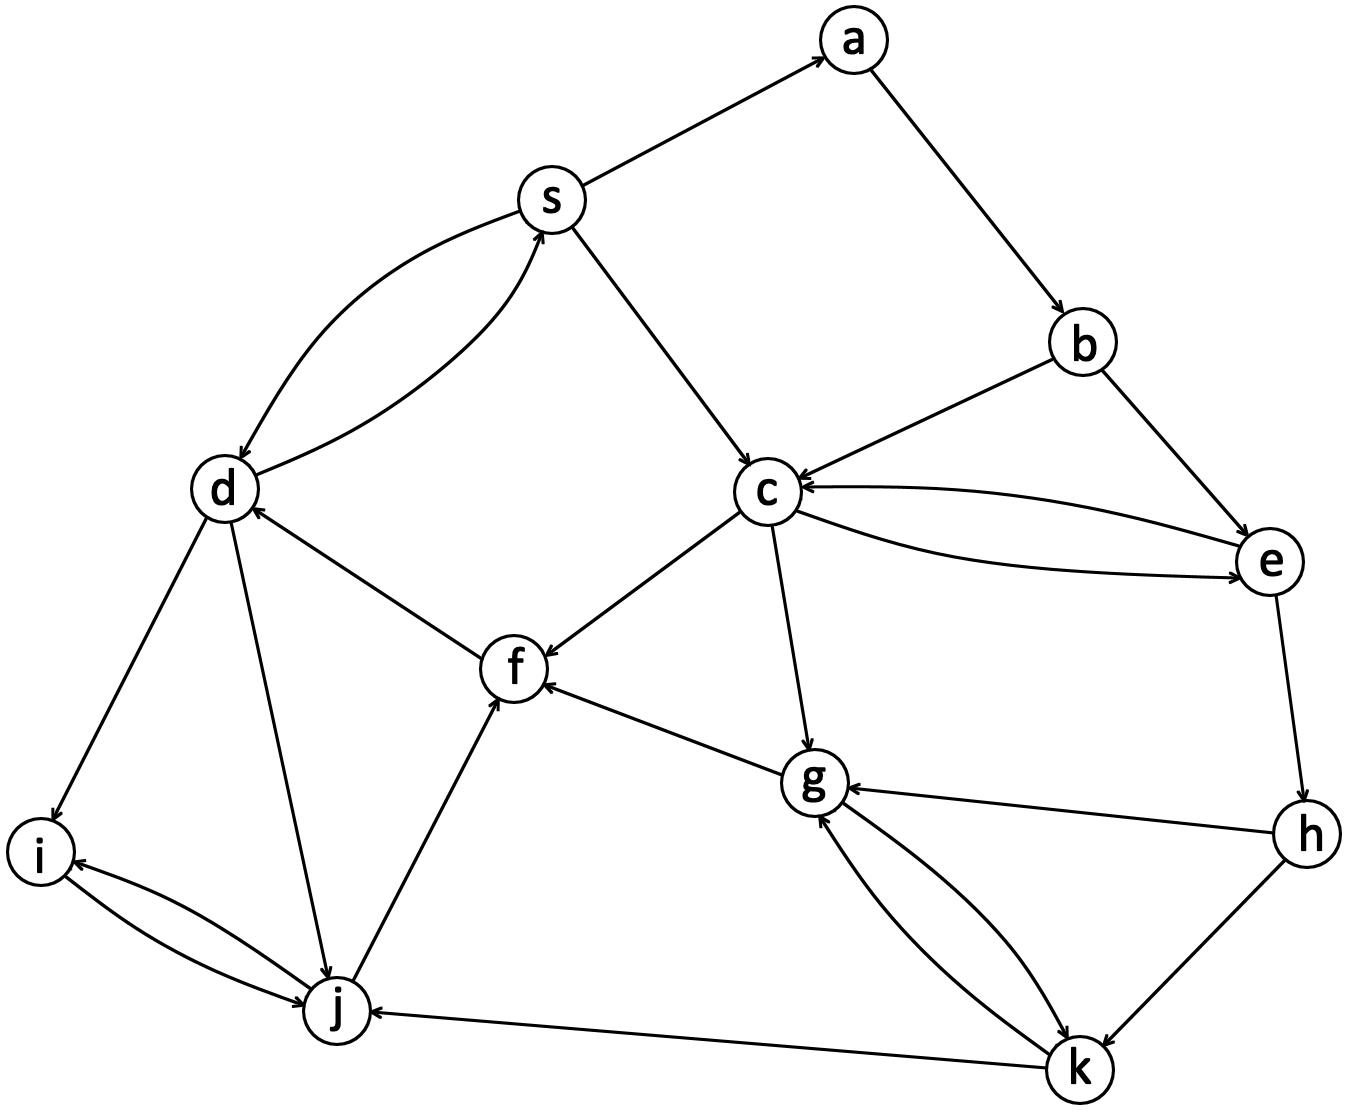
\includegraphics[height=6cm]{beispielgraph-edited}
	\end{figure}
\end{frame}

\begin{frame}{Graphen durchlaufen – Tiefensuche}
	\solutionheading
	Besuchsreihenfolge: \\ s, a, b, c, e, h, g, f, d, i, j, k
	\vspace{-.4\baselineskip}
	\begin{figure}[htp]
		\centering
		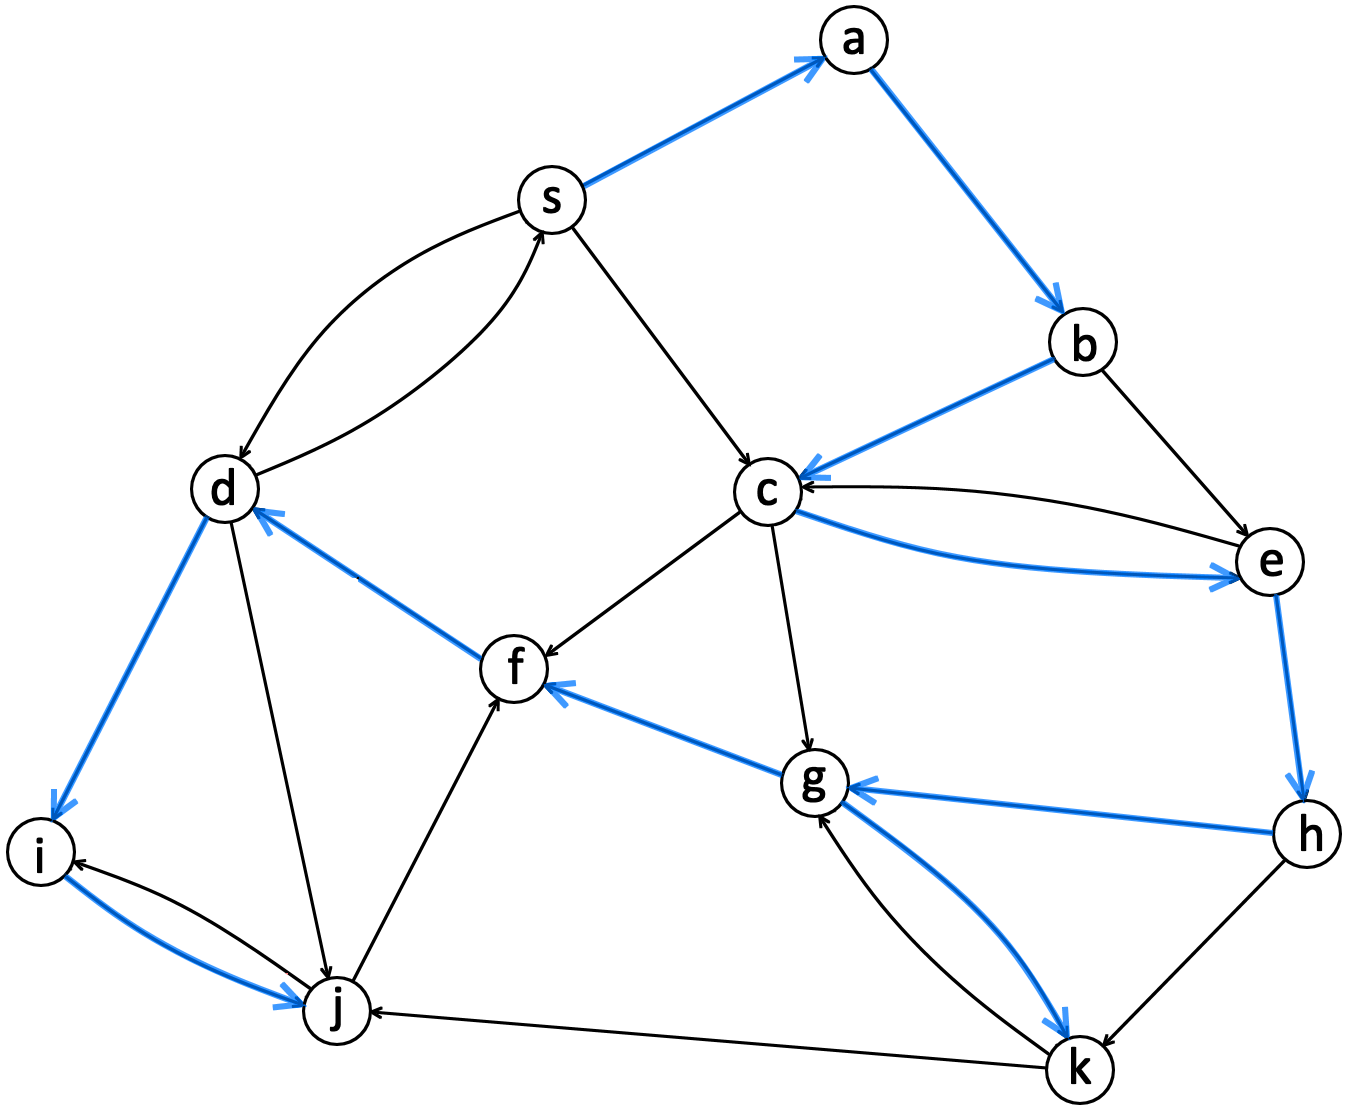
\includegraphics[height=6cm]{beispielDFS-edited}
	\end{figure}
\end{frame}

\begin{frame}[t]{Graphen durchlaufen – Tiefensuche}
	\begin{itemize}
		\item<+-> \textbf{Beobachtung}: Dringt schnell \textbf{tief} in den Graphen ein, anstatt sich „auszubreiten“ (daher der Name)
		\item<+-> \textbf{Laufzeit}? \visible<+->{$\Theta(n+m)$} \\ 
		\NoQuestionE{In-place?}{(wegen $visited$, $parent$ und Rekursion)}
		\item<+-> Etwas chaotische Laufwege -- geht's auch organisierter?
	\end{itemize}
\end{frame}

\begin{frame}{Graphen durchlaufen – Breitensuche}
	\begin{exampleblock}{Organisierte Reihenfolge: Breitensuche (einfach)}
		\begin{algorithm}[H]
			\Procedure{BFS$(G = (V, E),\ s \in V)$} {
				$visited := (\KwFalse, ... , \KwFalse)$\;
				$Q := \llist{s} : \|Queue|$ \;
				\While{$Q \neq \emptyset$} {
					$u := Q.\text{popFront}()$\;
					\If{$\neg visited[u]$} {
						visit$(u)$ \RComment{Do something with u} \;
						$visited[u] := \KwTrue$\;
						\ForEach{$(u, v) \in E$} {
							$Q.\text{pushBack}(v)$\;
						}
					}
				}
			}
		\end{algorithm}
	\end{exampleblock}
\end{frame}

\begin{frame}{Graphen durchlaufen – Breitensuche}
	\vspace{-.3\baselineskip}
	\begin{exampleblock}{Organisierte Reihenfolge: Breitensuche \textbf{mit Layer-Counter} uvm.}
		\begin{algorithm}[H]
			\small \vspace{-.4\baselineskip}
			\Function{BFS$(G = (V, E),\ s \in V): (parent, d)$} {
				$visited := (\KwFalse, ... , \KwFalse), \quad \alert{parent := (\bot, ..., \bot), \quad d := (0, ..., 0)}$\;
				$Q := \llist{s},$ \quad \alert{$Q' := \emptyset$}  \RComment{Extra queue Q'} \;
				$\alert{parent[s] := s, \quad layer := 0}$ \;
				\While{$Q \neq \emptyset$} {
					$u := Q.\text{popFront}()$\;
					\If{$\neg visited[u]$} {
						visit$(u, \alert{layer})$  \RComment{Do something with u and layer} \;
						$visited[u] := \KwTrue, \quad \alert{d[u] := layer}$ \;
						\ForEach{$(u, v) \in E$} {
							\alert{$parent[v] := u$} \;
							$Q'.\text{pushBack}(v)$  \RComment{Append to next-queue Q'} \;
						} \vspace{-.2\baselineskip}
					}
					\alert{
						\If{$Q = \emptyset$}{ 
							$(Q, Q') := (Q', Q)$ \RComment{New layer, so swap queues} \;
							$layer\pp$ 
						}
					} \vspace{-.2\baselineskip}
				} \vspace{-.2\baselineskip}
			}
		\end{algorithm} \vspace{-.5\baselineskip}
	\end{exampleblock}
\end{frame}

\begin{frame}{Graphen durchlaufen – Breitensuche}
	\taskheading{Volle Breitseite}
	Führt auf diesem Graphen Breitensuche von $s$ ausgehend aus. Nachbarn werden in alphabetischer Reihenfolge besucht.
	\vspace{-.3\baselineskip}
	\begin{figure}[htp]
		\centering
		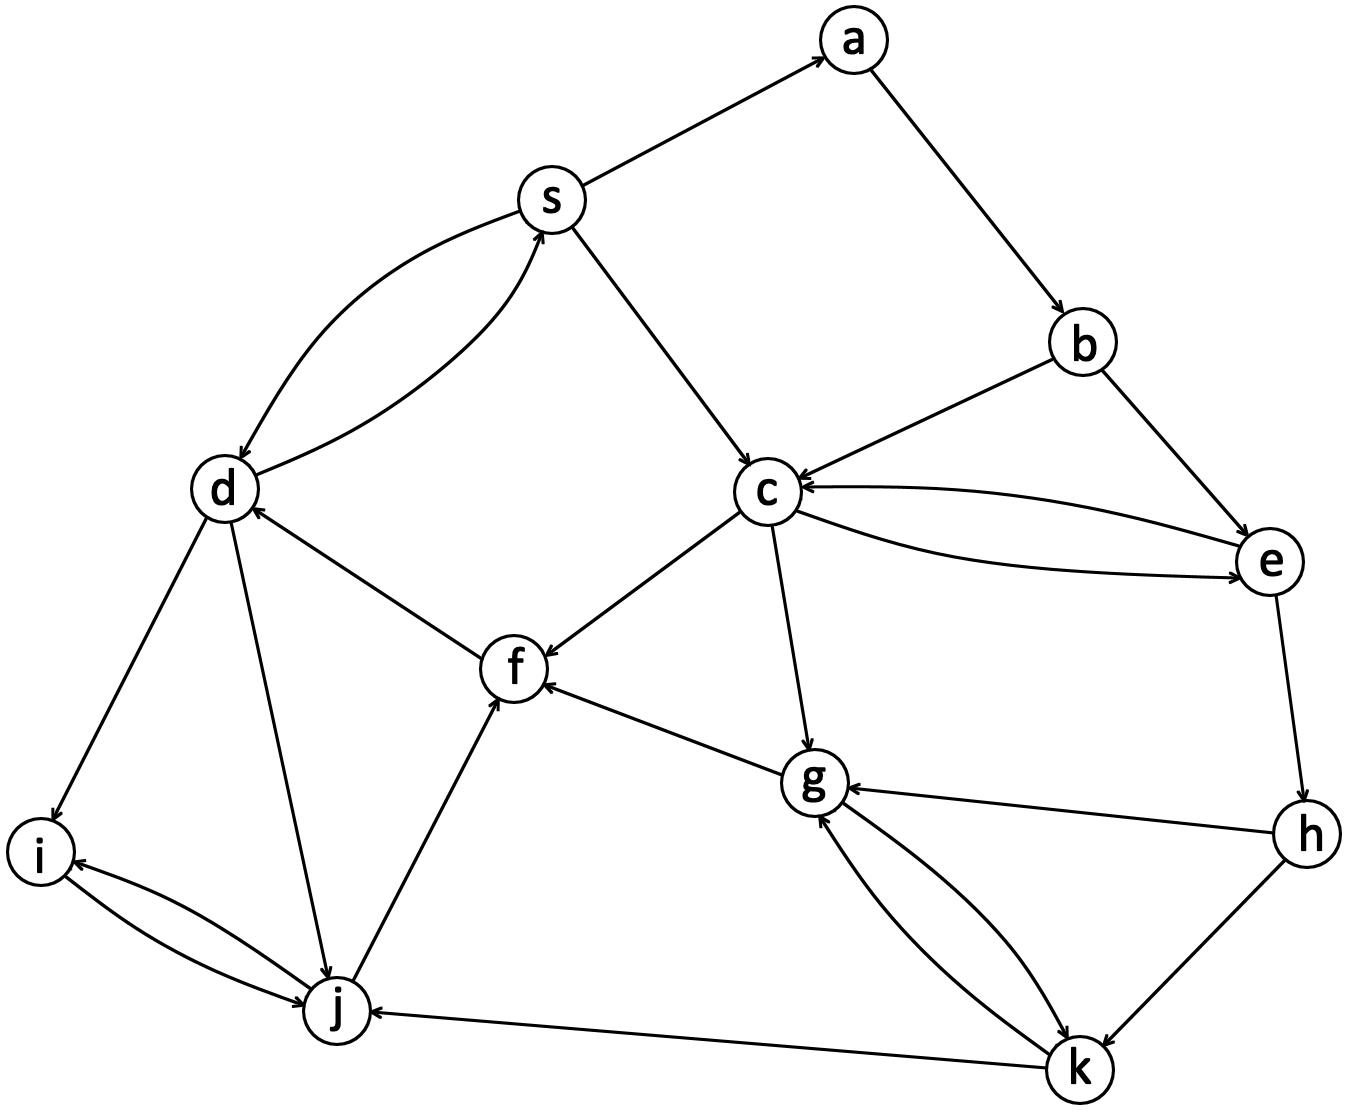
\includegraphics[height=6cm]{beispielgraph-edited}
	\end{figure}
\end{frame}

\begin{frame}{Graphen durchlaufen – Breitensuche}
	\solutionheading
	Besuchsreihenfolge: \\ s,\quad a, c, d, \quad b, e, f, g, i, j, \quad h, k
	\vspace{-.3\baselineskip}
	\begin{figure}[htp]
		\centering
		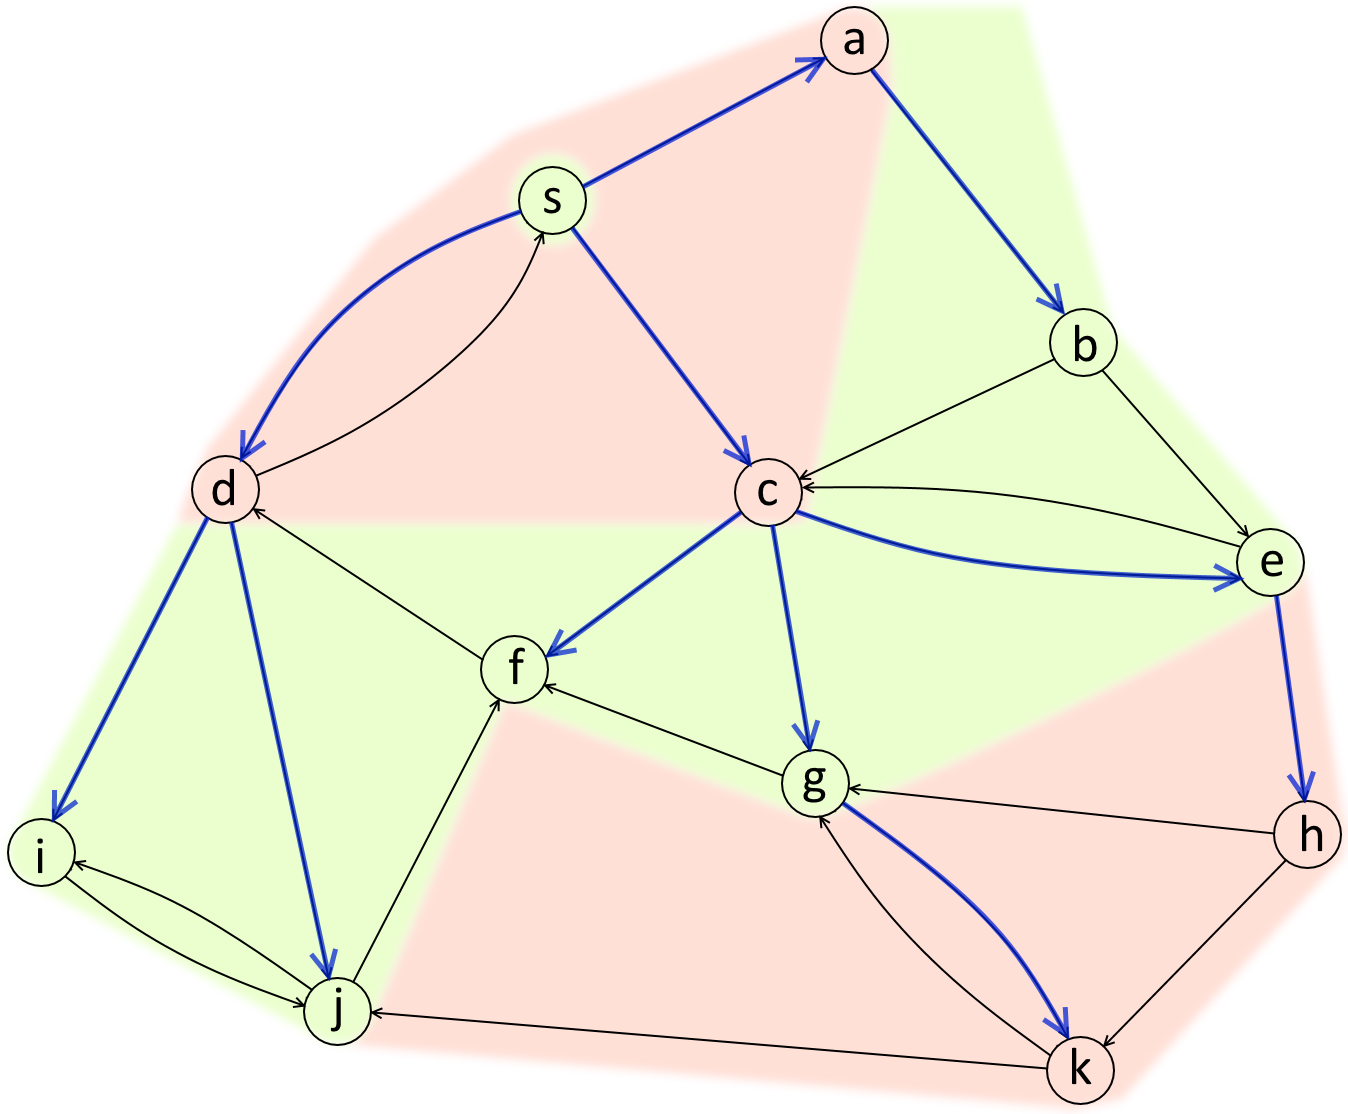
\includegraphics[height=6cm]{beispielBFSwithLayers}
	\end{figure}
\end{frame}

\begin{frame}{Graphen durchlaufen – Breitensuche}
	\begin{itemize}
		\item<+-> \textbf{Beobachtung}: \textbf{Breitet} sich schnell stark \textbf{aus} (daher der Name)
		\item<+-> Offensichtlich: Findet \textbf{kürzeste Pfade} (bei \textbf{ungewichteten} Kanten)
		\item<+-> \textbf{Laufzeit}? \visible<+->{$\Theta(n+m)$} \\ 
		\NoQuestionE{In-place}{(wegen $visited$, $Q$ und $Q'$)}
	\end{itemize}
\end{frame}

\begin{frame}{Graphen durchlaufen – Generell}
	\begin{itemize}
		\item DFS/BFS finden \textbf{Pfade} von Startknoten $s$ zu allen anderen erreichbaren Knoten \\
		\impl $parent$-Array zum Rekonstruieren der Pfade \\
		{\small ($parent[v]$: Vorgänger von $v$ im Pfad zu $v$)}
		\item DFS/BFS messen „\textbf{Distanz}“ der Knoten \\
		\impl $d$-Array mit $d[v] = $ Anzahl Kanten auf dem Weg zu $v$ 
		\implitem \textbf{Rückgabewerte} von BFS/DFS im Pseudocode benutzbar: \\
		$(parent, d) := \|BFS|(G, s)$ \RComment{DFS similar} \\
		\LComment{Now use $parent[\cdot]$ and $d[\cdot]$} 
		\bigskip
		\pause
		\item DFS/BFS finden \textbf{nur} alle von $s$ \textbf{erreichbaren} Knoten
		\implitem Um den \textbf{ganzen Graphen} abzudecken, müsst ihr von jedem noch nicht erreichten Knoten \textbf{extra} loslaufen \: \emph{(„Tiefen-/Breitensuchwald“)}
	\end{itemize}
\end{frame}

\begin{frame}{Graphen durchlaufen – Kantentypen}
	\begin{itemize}
		\item Bei BFS/DFS „entlanggelaufene“ Kanten \textbf{bilden Baum} {\small (da kein Knoten zweimal besucht!)}
		\pause
		\implitem Teile Kanten ein:
	\end{itemize}
	\vspace{-\baselineskip}
	{\small \begin{description} 
			\setlength\itemsep{0pt} % Fuck U, LATEX!
			\setlength\topsep{0pt} 
			\setlength\parskip{0pt}
		\item[\textbf{tree}-:] „Entlanggelaufene“ Kanten des Baumes
		\pause
		\item[\textbf{cross}-:] Kanten \textbf{zwischen} versch. \textbf{„Ästen“} im Baum
		\pause
		\item[\textbf{backward}-:] Kanten, die \textbf{rückwärts} zu (einer/mehreren) \emph{tree}-Kanten laufen
		\pause
		\item[\textbf{forward}-:] Kanten, die \textbf{mehrere} \emph{tree}-Kanten „\textbf{überholen}“
	\end{description}}
	\vspace{-.5\baselineskip}
	\centering
	\visible<2->{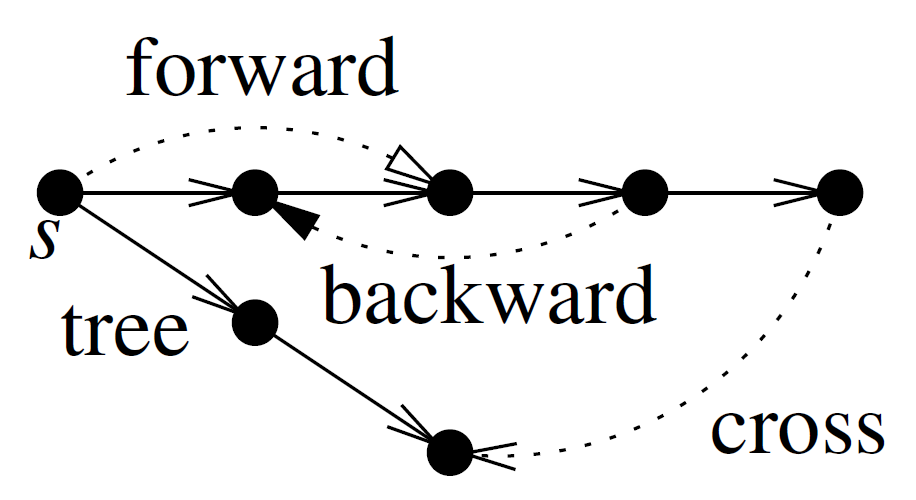
\includegraphics[width=.6\textwidth]{edgetypes}}
\end{frame}

\begin{frame}{Graphen durchlaufen – Kantentypen}
	\taskheading{Die Graphschaft besichtigen} 
	Betrachtet die vorhin durchgespielte Tiefen- und Breitensuche und klassifiziert jeweils alle Kanten entsprechend. \vspace{-.2\baselineskip}
	\begin{figure}[htp]
		\centering
		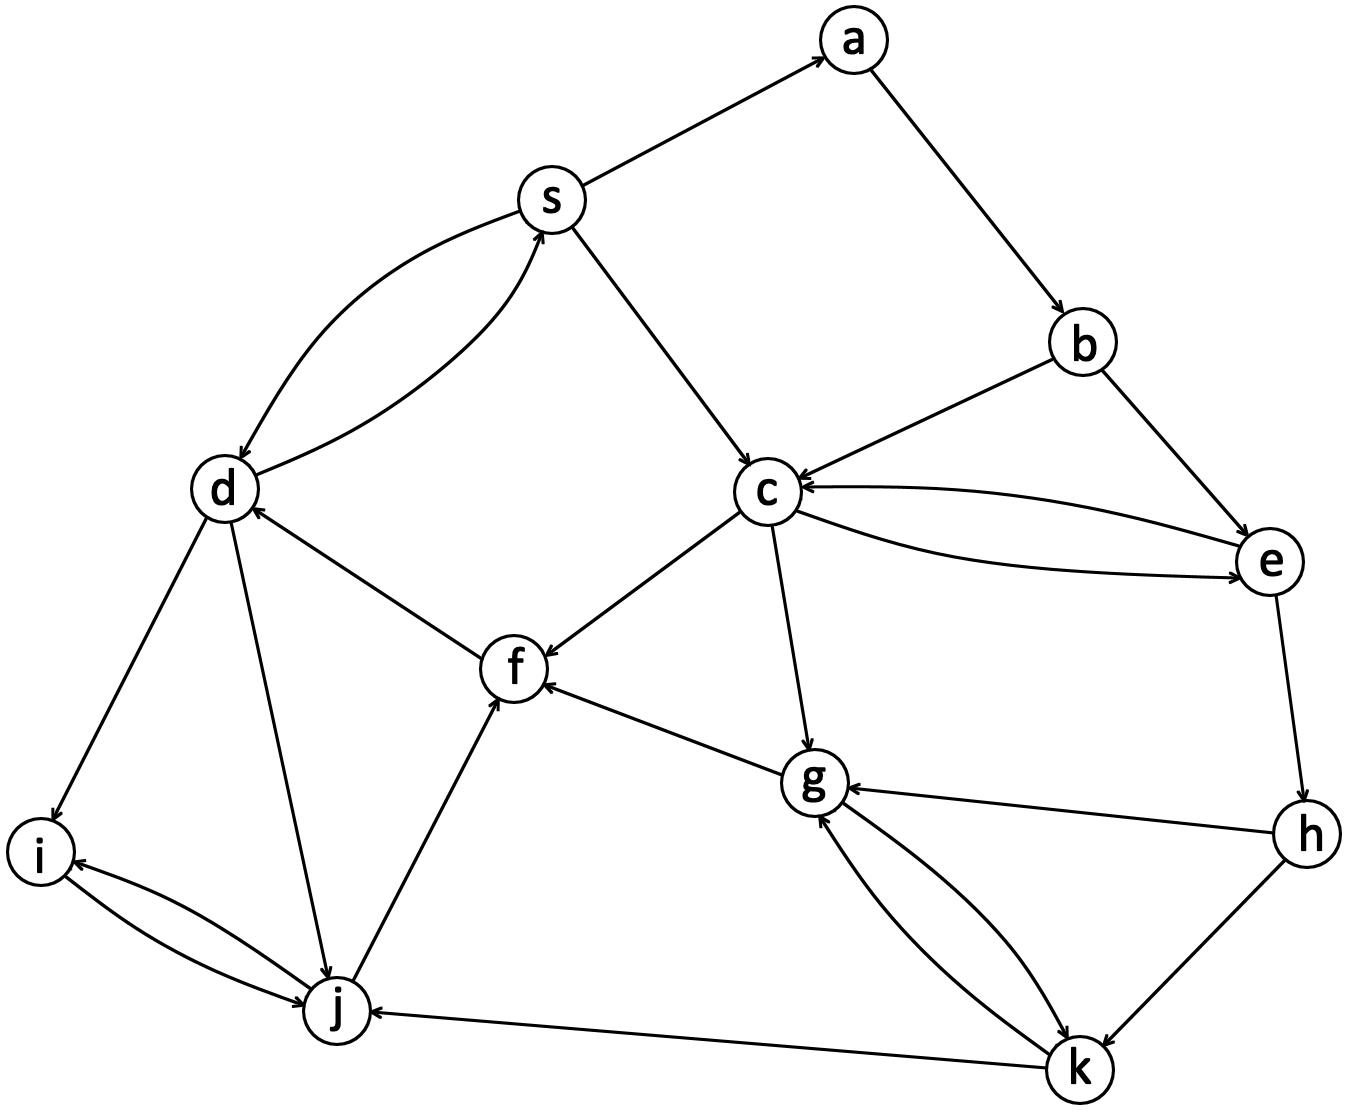
\includegraphics[height=6cm]{beispielgraph-edited}
	\end{figure}
\end{frame}

\begin{frame}{Graphen durchlaufen – Kantentypen}
	\solutionheading
	Für Tiefensuche: \\
	\vspace{-.3\baselineskip}
	\begin{figure}[htp]
		\centering
		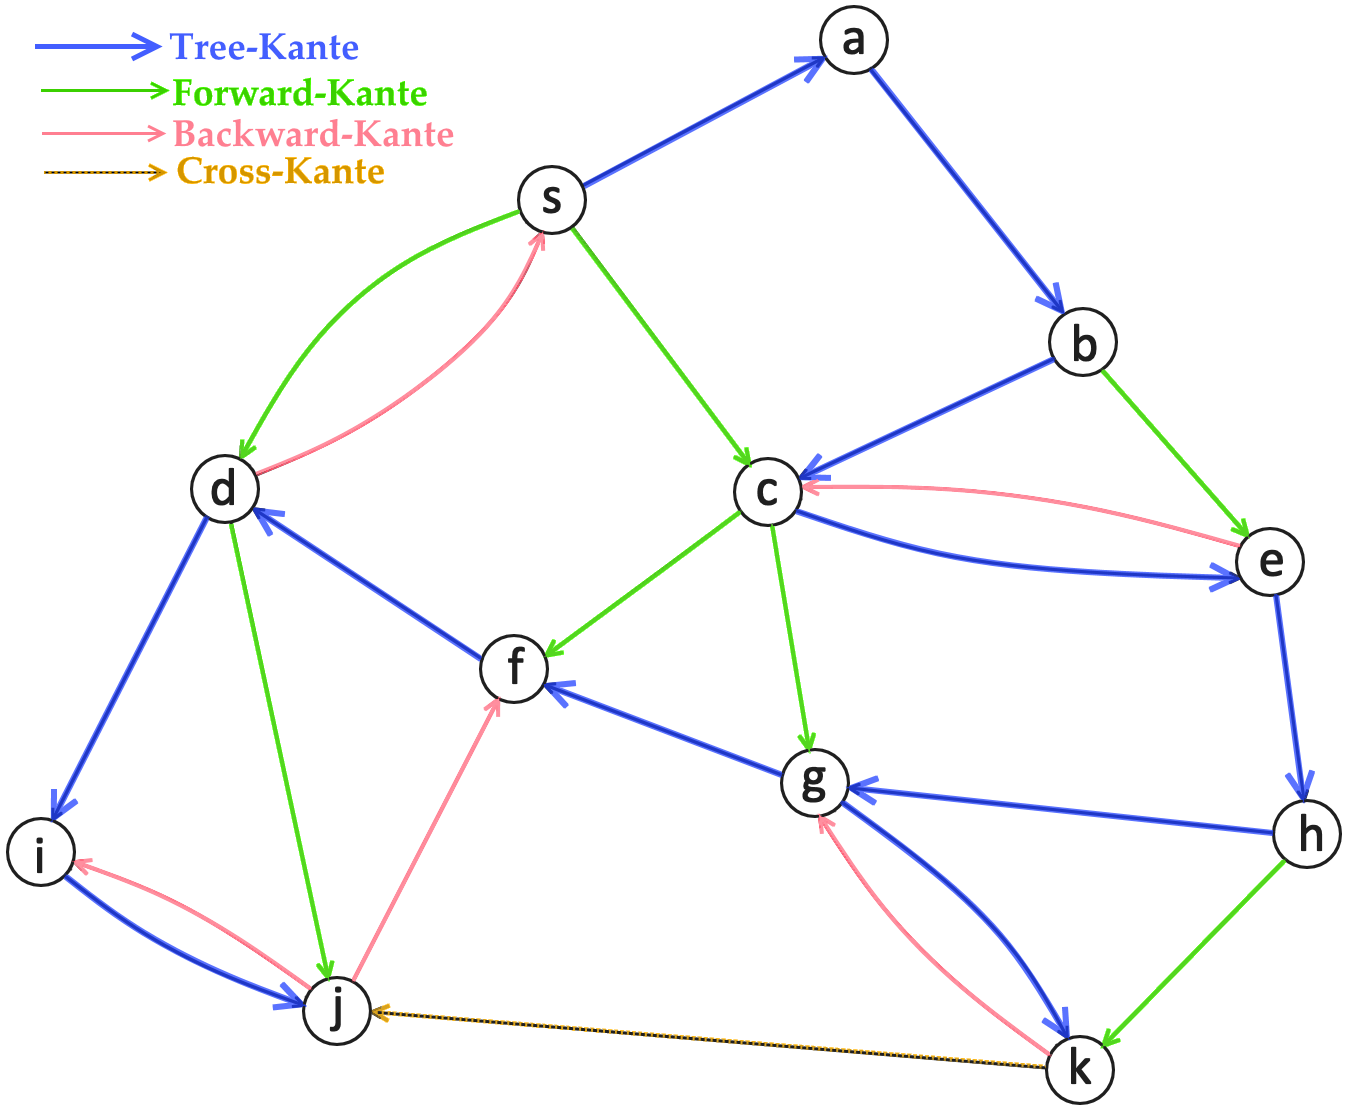
\includegraphics[height=6.5cm]{beispielDFStree-edited}
	\end{figure}
\end{frame}

\begin{frame}{Graphen durchlaufen – Kantentypen}
	\solutionheading
	Für Breitensuche:
	\vspace{-.3\baselineskip}
	\begin{figure}[htp]
		\centering
		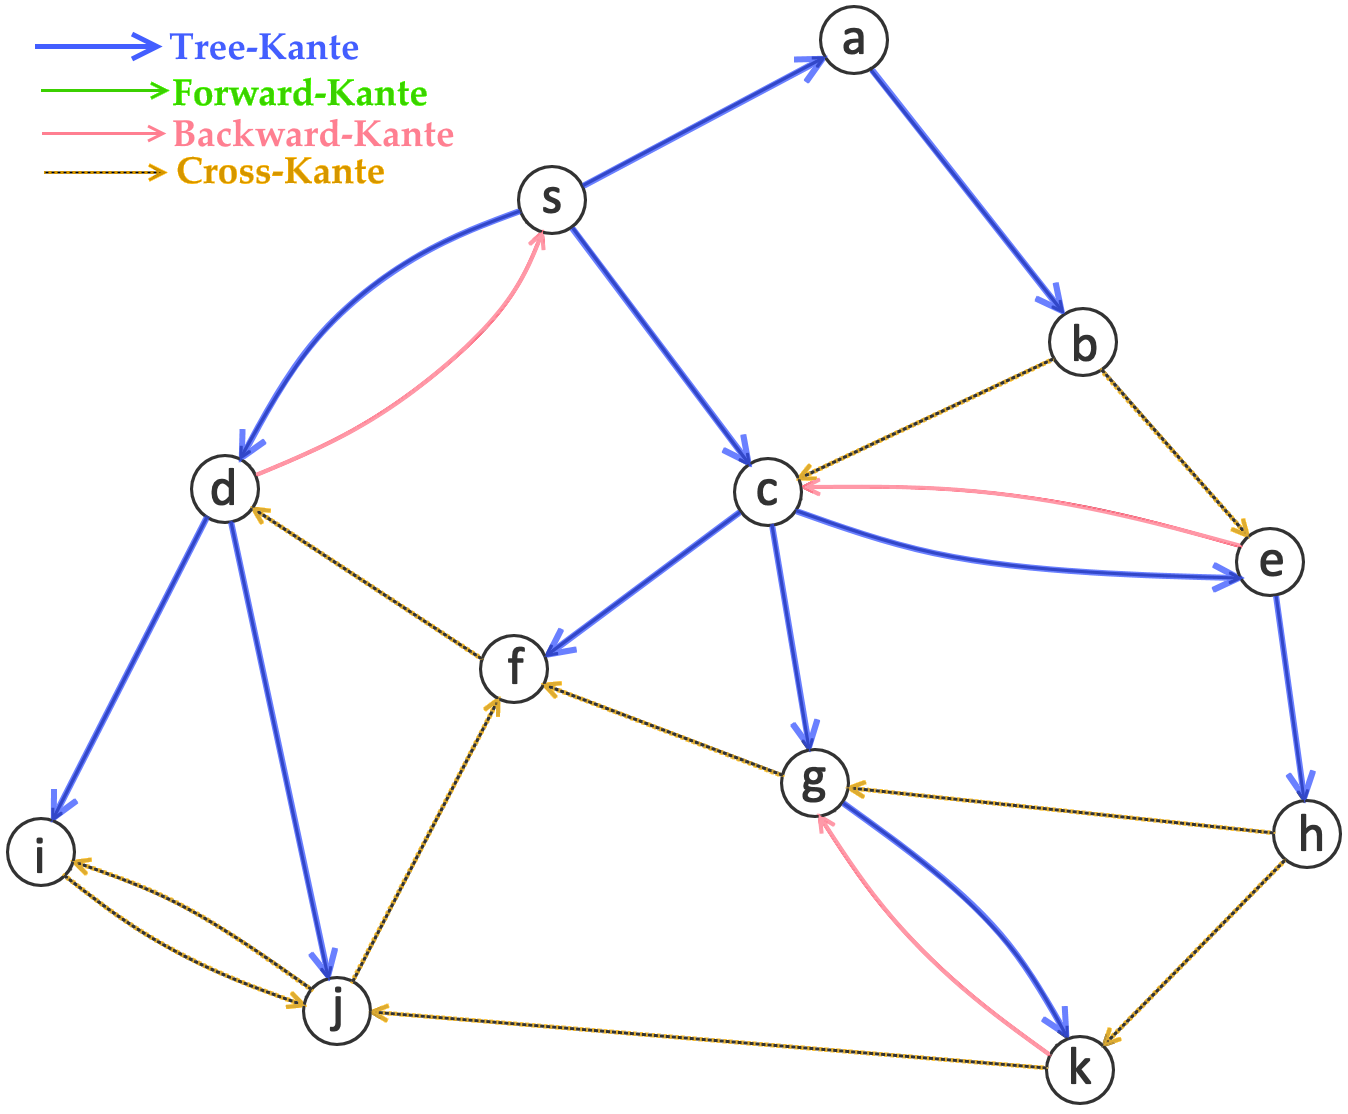
\includegraphics[height=6.5cm]{beispielBFStree-edited}
	\end{figure}
\end{frame}

\begin{frame}{Graphen durchlaufen – Kantentypen}
	\begin{itemize}
		\item Gibt es eine Art von Kante, die bei Breitensuche nicht auftreten kann? Falls ja, warum?
		\pause
		\implitem \textit{forward}-Kanten können \textbf{nicht} auftreten \\
		(BFS bestimmt schon den Pfad mit kleinster Kantenanzahl)
	\end{itemize}
\end{frame}

\begin{frame}{Graphen durchlaufen – Kantentypen}
	\begin{itemize}
		\item Gibt es eine Art von Kante, die bei Tiefensuche nicht auftreten kann? Falls ja, warum?
		\pause
		\item Bei Tiefensuche können \textbf{alle} Arten von Kanten auftreten.
	\end{itemize}
\end{frame}

\begin{frame}{Graphen durchlaufen – Kantentypen}
	\begin{itemize}
		\item Gibt es eine Art von Kante, die bei Tiefensuche \textbf{auf ungerichteten Graphen} nicht auftreten kann? Falls ja, warum?
		\pause
		\item \emph{cross}-Kanten können nicht auftreten: \\
		Wäre nämlich schon \textbf{vorher} entlanggelaufen worden (da ungerichtet!). Die einzigen Kanten, die hier das Ende eines Tiefensuch-Astes markieren können, sind \emph{backward}-/\emph{forward}-Kanten. \\
		(Ob man die jetzt \emph{backward}- oder \emph{forward}- nennt, ist wurscht, sind ja faktisch \textbf{beides}.) Bsp. dazu:
	\end{itemize}
	\centering
	\visible<2->{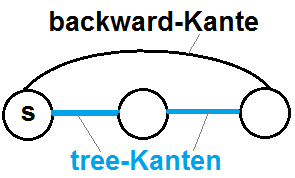
\includegraphics[width=.35\textwidth]{backward-dfs-undirected}}
\end{frame}

\begin{frame}{Graphen durchlaufen – Kantentypen}
	\begin{itemize}
		\item Sind \emph{cross}-Kanten eindeutig? Falls ja, warum?
		\pause
		\item \emph{cross}-Kanten sind genau dann eindeutig, wenn der zugehörige Baum eindeutig ist. \impl I.~A. \textbf{nicht} der Fall (da Nachbarn i.~A. nicht in bestimmter Reihenfolge gewählt).
	\end{itemize}
\end{frame}

\begin{frame}{Graphen durchlaufen – Kantentypen}
	\begin{itemize}
		\item Nach welcher Strategie muss bei Tiefensuche die Reihenfolge der rekursiven Abstiege (also die Reihenfolge der Nachbarn) gewählt werden, damit keine \textit{forward}-Kanten auftreten?
		\pause
		\item \textbf{Fangfrage}! :P \\
		Es gibt \textbf{keine} solche Strategie; \emph{forward}-Kanten bei DFS in manchen Fällen unvermeidbar
	\end{itemize}
\end{frame}	


% Theoretisch prokrastinierbar, aber weils hier thematisch besser passt... Zeit langt vermutl. eh nicht:

\begin{frame}{Graphen durchlaufen}
	\taskheading{Tiefensuche revisited} 
	Implementiert Tiefensuche nicht-rekursiv als Pseudocode. Das asymptotische Laufzeitverhalten von eigentlicher Tiefensuche darf hierbei nicht überschritten werden.
\end{frame}

\begin{frame}{Graphen durchlaufen}
	\solutionheading
	Recursion-Faking mittels Stack: 
	\begin{algorithm}[H]
		\Procedure{DFS$\left(G=(V,E),\ s \in V\right)$}{
			$S := \llist{s} : \text{Stack}$ \;
			$visited := (\KwFalse, ..., \KwFalse)$ \;
			\While{$S \neq \emptyset$}{
				$u := S$.popBack$()$ \;
				\If{$\neg visited[u]$}{
					visit$(u)$ \RComment{Do something with u} \;
					$visited[u] := \KwTrue$ \; 
					\ForEach{$(u,v) \in E$}{
						$S$.pushBack$(v)$ \;
					}
				}
			}
		}
	\end{algorithm}
	\vphantom{\impl Tp}
\end{frame}

\begin{frame}{Graphen durchlaufen}
	\solutionheading
	Zum Vergleich: Breitensuche mit Queue
	\begin{algorithm}[H]
		\Procedure{BFS$(G = (V, E),\ s \in V)$} {
			$\alert{Q} := \llist{s}: \alert{\|Queue|}$ \;
			$visited := (\KwFalse, ... , \KwFalse)$\;
			\While{$\alert{Q} \neq \emptyset$} {
				$u := \alert{Q}.\text{pop\alert{Front}}()$\;
				\If{$\neg visited[u]$} {
					visit$(u)$ \RComment{Do something with u} \;
					$visited[u] := \KwTrue$\;
					\ForEach{$(u, v) \in E$} {
						$\alert{Q}.\text{pushBack}(v)$\;
					}
				}
			}
		}
	\end{algorithm}
	\impl Der Apfel fällt nicht weit vom Tiefensuchbaum... :P
\end{frame}



\xkcdframevert{761}{}{1.5}

\only<beamer:0>{\slideThanks}

\end{document}